\chapter{The blood microbiome}

\section{Importance of the microbiome}

The colon of an adult human contains approximately $10^{14}$ micro-organisms, which outnumber host cell numbers by up to two orders of magnitude and house at least 100-fold more bacterial genes than human \cite{Brenchley:2012bm}. The importance of the microbiome has become evident in part through studies of germ-free animals: these animals have reduced vascularity, digestive enzyme activity, and muscle wall thickness. Furthermore, numerous human studies have implicated changes in microbial composition (dysbiosis) with many diseases, such as obesity, celiac disease, type 2 diabetes, atopic eczema, asthma, inflammatory bowel disease, and chronic diarrhea  \cite{Brenchley:2012bm}.

\section{Linking blood and body sites}

The Human Microbiome Project defined the compositional range of the microbiome within healthy individuals \cite{Consortium:2012bb}. Since this pioneering work, there has been great interest in studying changes in the microbiome  across different physiological contexts. Pregnancy is one example, as preterm birth is a leading cause of neonatal mortality and can be driven by intrauterine infections. Until recently, it was thought that intrauterine infections originated in the lower genital tract and microbiota ascended into the otherwise sterile womb \cite{Prince:2014gx}. Recent studies have shown that the microbiome changes during pregnancy according to hormonal and physical fluctuations \cite{Koren:2012ji}. In addition, the human placenta is not sterile, but rather harbors a unique microbiome with taxonomic composition similar to the oral cavity. The work suggested that transmission of micro-organisms from various body sites, potentially via blood, may help to seed (or alter the composition of) the placental microbiome \cite{Aagaard:2014vk}. 

\begin{figure*}
\center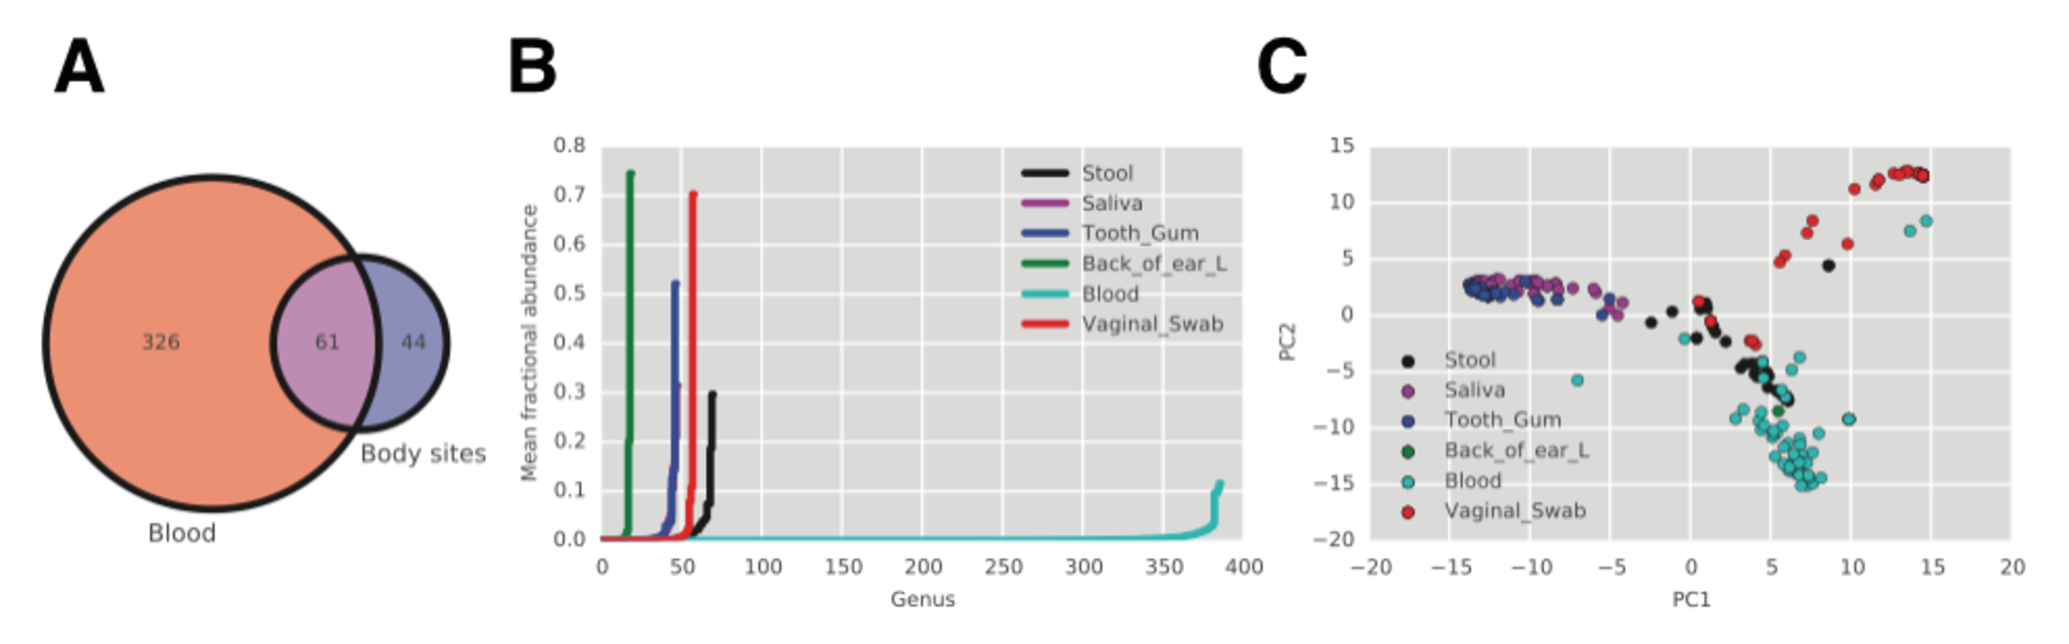
\includegraphics[width=160mm,scale=0.5]{Figures/Fig12}
\caption{Composition of the blood microbiome}
\label{fig:Fig12}
\end{figure*}

Due to the apparent connection between the microbiome, blood, and fetal health, pregnancy is an interesting context for examining the linkage between the microbiome at body sites relative to blood. Recent work has shown that micro-organism derived cell-free DNA fragments can be purified from blood and counted using next-generation sequencing (NGS) \cite{DeVlaminck:2013hl}. Much of this material is likely to be the detritus of dead and apoptosed cells \cite{Quake:2012iy}, which has leaked from tissues into the blood.  

We examined the composition of these micro-organism derived cell-free DNA fragments recovered from blood relative to four commonly sampled body sites (Saliva, Vagina, Gut, and Gum) within a cohort of fourteen pregnant women enrolled in a clinical study at Stanford hospital.  We performed shotgun sequencing of cell-free DNA collected from fifty eight plasma samples. For each sample, we performed temporally matched 16s sequencing on the four body sites.

We first performed descriptive analysis of the data by comparing the taxonomic composition of blood relative to the sampled body sites at genus-level resolution. We discretized mean fractional abundance data for blood and all sampled body sites, resulting in a binary value for each genus. We then compared the genus detected in blood to genus detected in body sites. $58$\% of the genus detected in the body sites were also found in blood, while only $15$\% of the genus detected in blood were detected in any body site. This suggested that micro-organism derived material in blood originates from more than just the sampled sources.

We then evaluated the distribution of mean fractional abundances for each body site relative to blood. The 16s sampled body sites showed strong enrichment in particular genus that are known to be well-adapted to each niche \cite{Consortium:2012bb}. Blood is quite different: the number of genus detected is $\approx 8$-fold greater than the body sites, with a mean fraction abundance $\approx 10$-fold lower. We transformed the data using PCA in order to determine the genus that most strongly explain the variation between samples for all tissues (Figure ~\ref{fig:Fig12}). The body sites cluster together in the transformed space, as expected, and blood occupies a distinct compositional niche relative to the sampled body sites. We examined genus that strongly contribute to the principal components in order to understand what genus distinguish blood from the body sites: as expected, genus that explain variation in blood relative to the sampled body sites (notably, Acidovorax and Cupriavidus) have the among the highest fraction abundance in blood, but are absent from the sampled body sites. 

We next examined whether blood samples from each body site. Body-site specific micro-organisms provide a reasonable indicator for this. In turn, we computed specificity by discretizing the genus found in each body site and comparing discretized data for each body site to discretized data for all other sites (Figure ~\ref{fig:Fig13}). For this analysis, we used our sampled body site data as well as the metagenomic community profiles made available by the Human Microbiome Project \cite{Consortium:2012bb}, which contain 690 samples from 300 US subjects across 15 body sites. 

In both cases, we computed a list of specific genus, which were only detected in single body sites for all samples collected in either study. We then asked whether these genus were detected in our blood measurements: we detected $57$\% and $45$\% of the site-specific genus in blood determined via HMP metagenomic community profiles and the 16s data collected for this study, respectively. We found no significant difference between the abundance of site specific genus detected in blood versus theses un-detected, which argues against the possibility that technical limitations (e.g., under-sampling) explain the detection failure.

\begin{figure*}
\center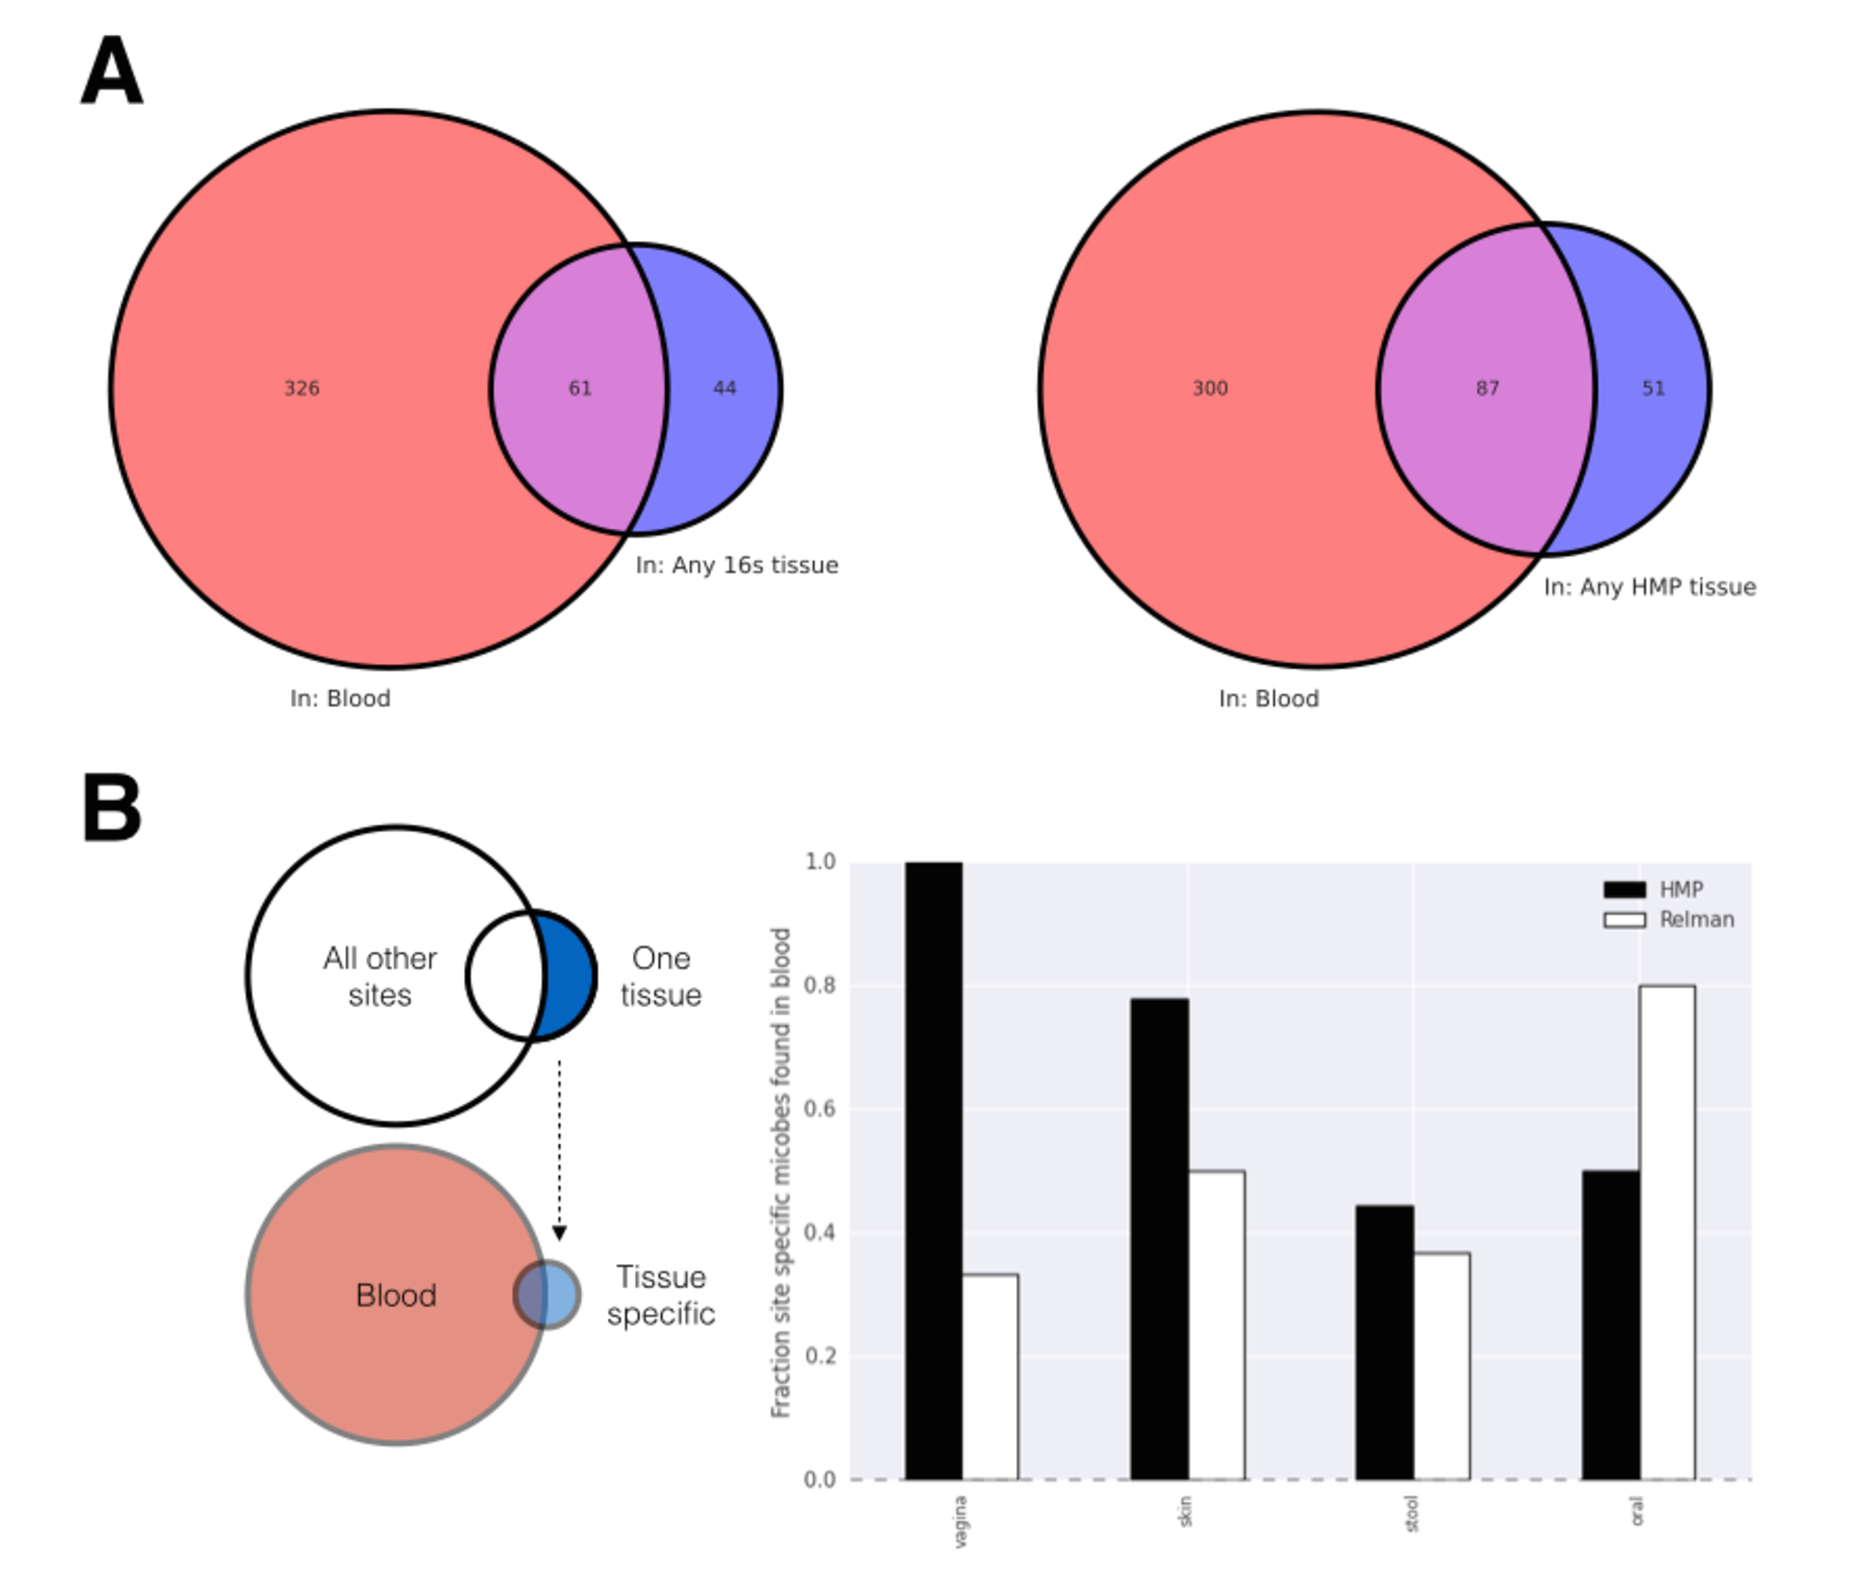
\includegraphics[width=150mm,scale=0.5]{Figures/Fig13}
\caption{Detection of body site specific bacteria in blood.}
\label{fig:Fig13}
\end{figure*}

From the results of analysis, we obtained an assignment of body site specificity for each genus in our data; each genus was either assigned to a specific body site or not, the latter indicating that it was detected in more than one body site. We partitioned the genus detected in blood using this assignment and aggregated fractional abundance within each partition. This analysis indicated that blood is composed primarily of micro-organisms with two likely source: genus derived from mixed sources, which cannot be traced to any specific tissue, and genus that are only detected in blood (Figure ~\ref{fig:Fig14}a). The 20 most abundant genus detect in blood (Figure ~\ref{fig:Fig14}b) were either exclusive to blood or originate from mixed sources. 

\begin{figure*}
\center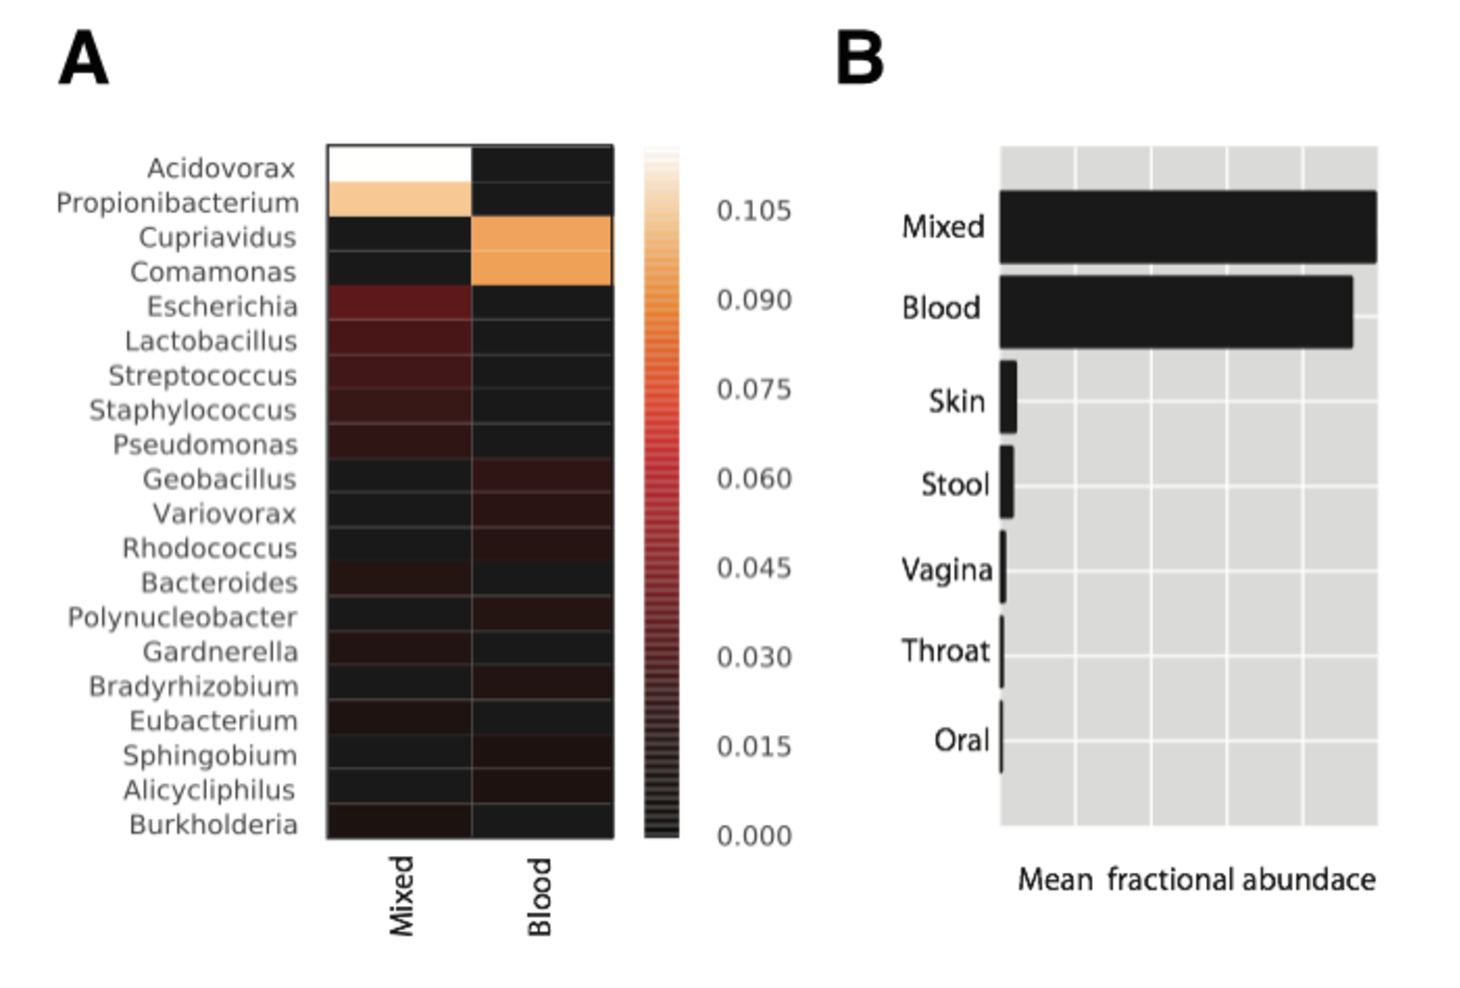
\includegraphics[width=150mm,scale=0.5]{Figures/Fig14}
\caption{Likely sources for most abundant bacteria detected in blood.}
\label{fig:Fig14}
\end{figure*}

\section{Coupling between blood and body sites}

We then asked if a physical relationship between genus found in blood and  body sites can be established. Specifically, we examine whether the fractional abundance of genus at any body site is linked to its detection in blood. In order to do this, we discretized the blood data for each sample. For each genus, we then evaluated the fractional abundance of that genus for all matched body site samples. We compared the distribution of abundances at each body site based upon whether the genus was found in blood, expecting a difference in distribution if a body site was detectably coupled to blood (e.g., an elevation in abundance at a tissue when the genus was found in blood). However, found no signifiant difference between the body site fractional abundance with respect to detection in blood. 

We further examined whether the composition of genus detected in blood can be modeled as a function of the sampled sites. We took a simple approaching, choosing a linear model. This assumes that each blood sample is a linear combination of the genus at temporally matched body sites. We used a quadratic programming package in order to determine the mixing coefficients that minimize the squared error between the model output and the actual blood measurement subject to intuitive constraints (e.g., the coefficients must be greater than zero). After confirming the solver works correctly by recapitulating the correct mixing coefficients on simulated data, we applied this approach to all blood samples with matched body site data.

\begin{figure*}
\center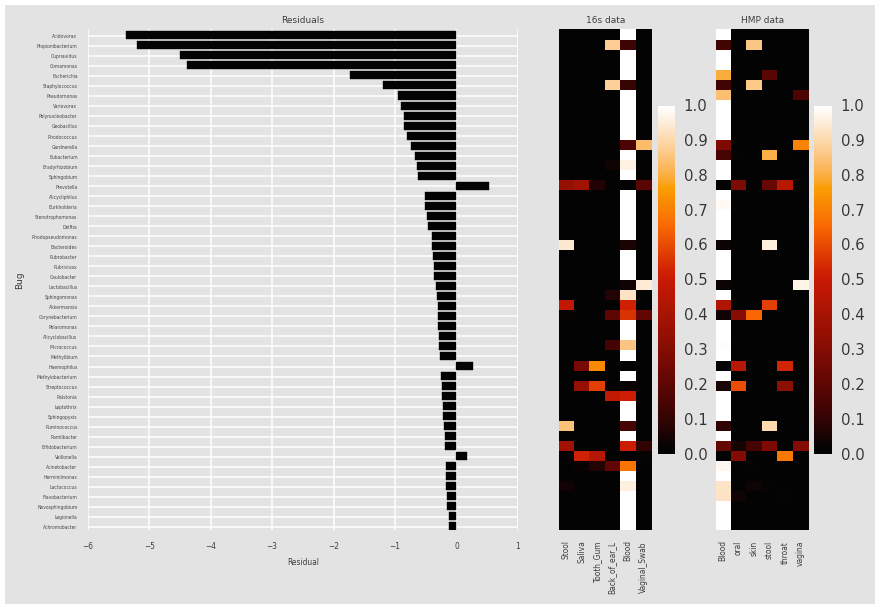
\includegraphics[width=150mm,scale=0.5]{Figures/Fig14_2}
\caption{Residuals from linear regression.}
\label{fig:Fig14_2}
\end{figure*}

We found that the model performed poorly, using coefficient of determination ($r^2$) between the model guess and actual blood data as a measure of fit. However, examination of the the residuals was informative: intuitively, we found that the model fails because many highly abundant genus detected in blood are not found in the sampled body sites. In order words, the sampled sources are insufficient to describe the composition of blood, as blood apparently samples from additional tissues or serves as an environment that amplifies specific genus non-linearly.

\section{Summary}

The abundance distribution of genus measured in blood differs from the sampled body sites. Body sites are dominated by few genus with high fractional abundance and have short tail of low-abudnance genus. This likely reflects the fact that specific genus are well-adapted to the niche provided by each body site  \cite{Consortium:2012bb}. In contrast, blood contains many more genus, but with long tail detected at trace abundance. In turn, blood may serve as a common sink into which all tissues contribute dead cells, resulting in a passive environment of mixed DNA fragments. Yet, we also found that most abundant genus in blood were absent from the sampled body sites. This suggests that that blood is either dominated by genus contributed by body sites that were un-sampled or that blood may is a niche for these genus.

Analysis of site-specific genus provides evidence that each sampled body site contacts blood. However, we did not observe a significant relationship between the detection of a particular genus in blood and its abundance in any sampled body site. This may have several explanations. First, our sampling of micro-organism derived cell-free DNA fragments is limited by the high background of human derived signal. In turn, our sequencing depth of micro-orgaism derived fragments in blood may be insuficcient. Second, body site 16s measurements are normalized, resulting in a fractional abundance value for each detected genus. Yet, the microbial population sizes may differ considerably between body sites, meaning that fractional abundance may be poor indicator of the absolute contribution that a genus can make to blood. Finally, many body sites may be contributing similar genus to blood, obscuring the apparent linkage between abundance at any one site and the abundance in blood. This point is supported by our results from linear regression analysis: we detected many high abundance genus in blood that were not measured in any of the sampled sites. Thus, it is likely that additional sites contribute to blood. 

We have shown that blood contains several-fold more genus than body samples sampled using either 16s or metagenomic sequencing. Each sampled tissue contributed to blood, though the most abundant genus detected in blood appear to originate from un-sampled tissues. The depth of sequencing employed in prior studies has been sufficient to show a correlation between the abundance of micro-organism derived cell-free DNA and significant changes to the host, including deep tissue infection and immunocompetence \cite{DeVlaminck:2013hl}. Yet, this study suggests that depth of sequencing employed may be insufficient to establish a correlation between cell-free DNA and commensal micro-biome composition at the sampled sites. With deeper sequencing of blood along with more extensive profiling of the human microbiome, it may be possible to (1) explain the currently un-defined tissues of origin for many of micro-organisms detected in blood and (2) understand physical linkage between microbial abundance at body sites and blood.
